\section{Einleitung\label{spannung:section:Einleitung}}
\rhead{Einleitung}
Das Hook'sche Gesetz beschreibt die Beziehung von Spannung und Dehnung von linear-elastischen Materialien im Eindimensionalen.
In diesem Kapitel geht es darum das Hook'sche Gesetz im Dreidimensionalen zu beschreiben.
Durch variable Krafteinwirkungen entstehen in jedem Punkt des Materials eine Vielzahl an unterschiedlichen Spannungen.
In jedem erdenklichen Punkt im Dreidimensionalen herrscht daher ein entsprechender individueller Spannungszustand.
Um das Hook'sche Gesetz für den 3D Spannungszustand formulieren zu können, reichen Skalare nicht aus.
Darum werden Vektoren, Matrizen und Tensoren zur Hilfe gezogen.
Mit diesen lässt sich eine Spannungsformel für den 3D Spannungszustand bilden.
Diese Spannungsformel ist Grundlage für Computerprogramme und geotechnische Versuche, wie der Oedometer-Versuch.

Um die mathematische Untersuchung vorzunehmen, beschäftigt man sich zuerst mit den spezifischen Gegebenheiten und Voraussetzungen.
Ebenfalls gilt es ein paar wichtige Begriffe und deren mathematischen Zeichen einzuführen.
In diesem Kapitel gehen wir auch auf die Zusammenhänge von Spannung, Dehnungen und Verformungen an elastischen Materialien ein,
wie sie in gängigen Lehrbüchern der Mechanik oder der Geotechnik behandelt werden. z. B. [\cite{spannung:Grundlagen der Geotechnik}]

\section{Spannungsausbreitung\label{spannung:section:Spannungsausbreitung}}
\rhead{Spannungsausbreitung}
Die Geotechnik ist eine Ingenieurdisziplin, bei welcher man Erdbau und den Erdbau tangierende Bauwerke dimensioniert.
Sie beinhaltet aber auch die statische Beurteilung von Boden und Fels.

Belastet man den Boden mit einer Spannung
\[
\sigma
=
\frac{F}{A}
,
\]
so wird diese in den Boden geleitet und von diesem kompensiert.
Im Boden entstehen unterschiedlich hohe Zusatzspannungen.
Diese Zusatzspannung breitet sich räumlich im Boden aus.
Im Falle einer konstanten Flächenlast $\sigma$ (siehe Abbildung 1.1) breitet sich die Zusatzspannung zwiebelartig aus.

\begin{figure}
	\centering
	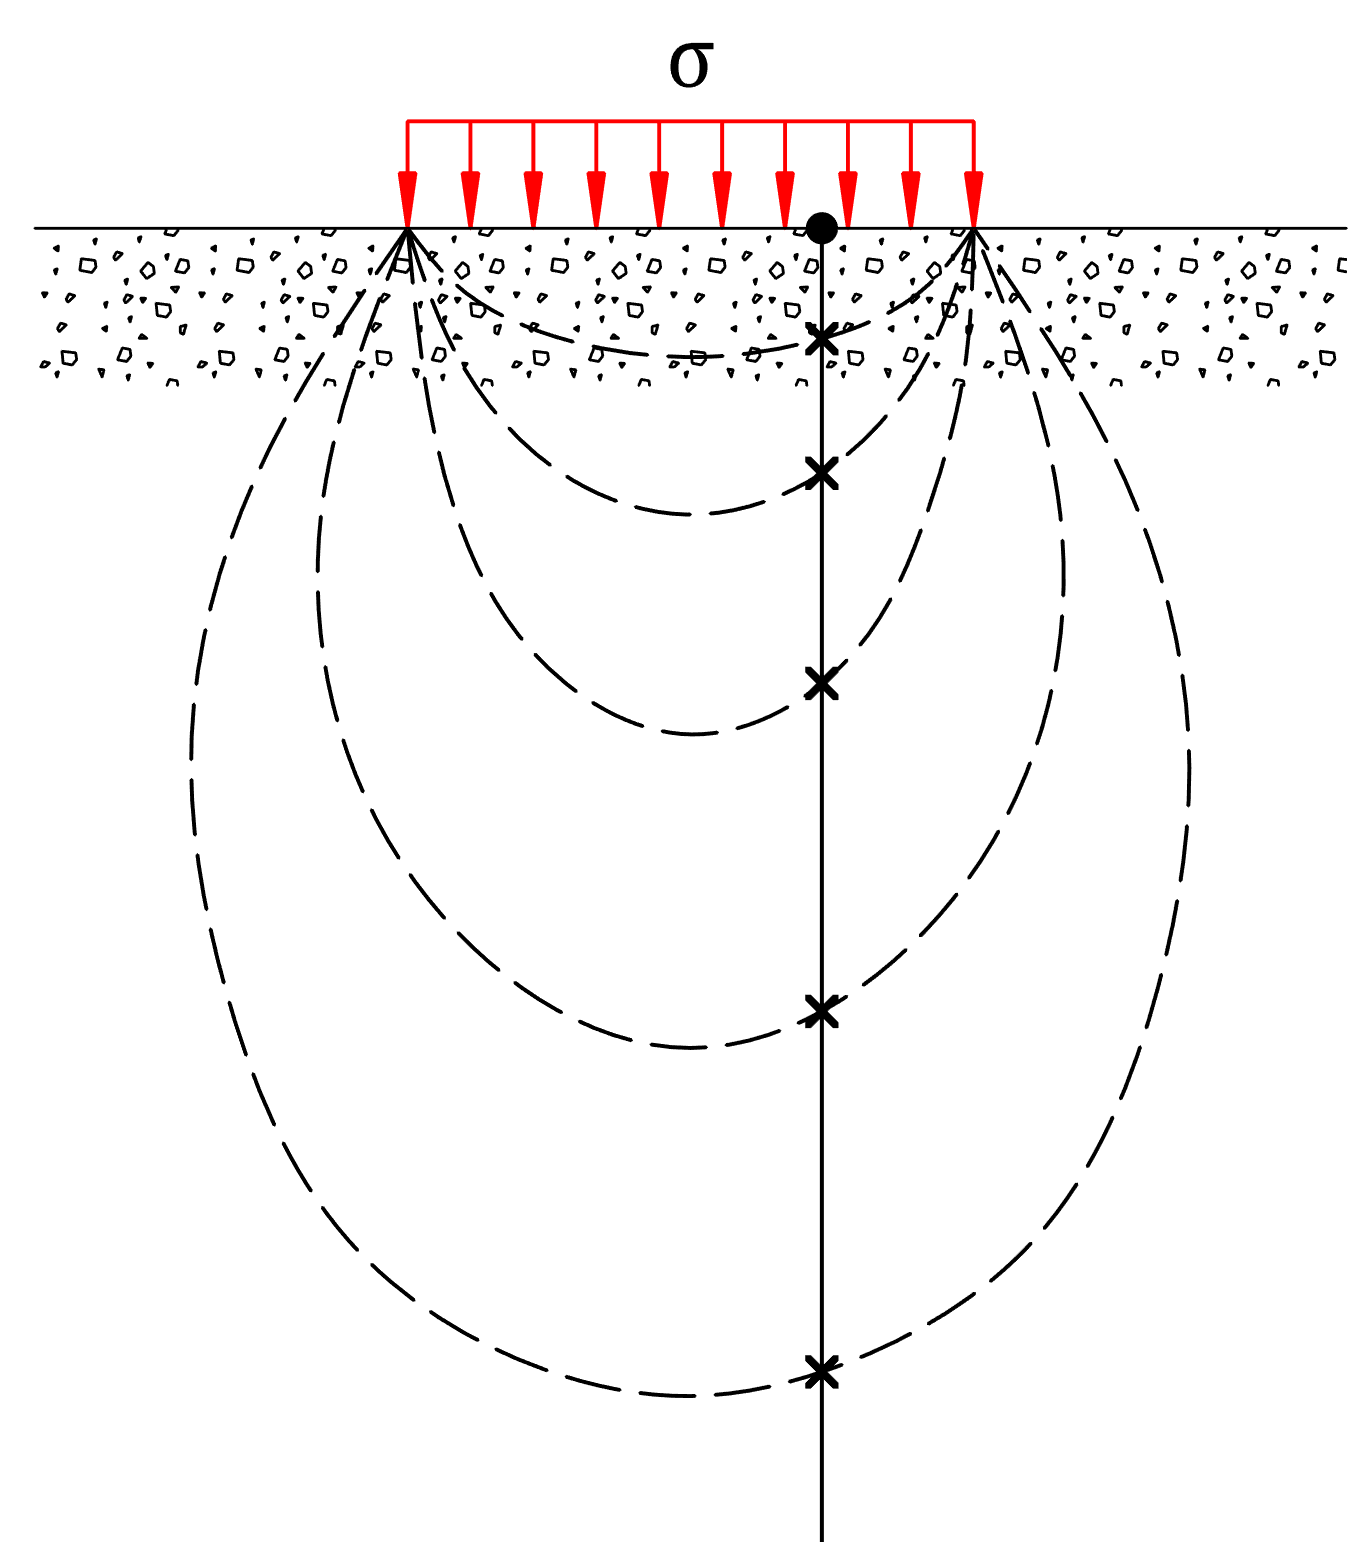
\includegraphics[width=0.4\linewidth,keepaspectratio]{papers/spannung/Grafiken/Bild4.png}
	\caption{Ausbreitung der Zusatzspannung im Boden infolge einfacher Flächenlast}
	\label{fig:Bild4}
\end{figure}

Mit der Tiefe $t$ nimmt diese permanent ab (siehe Abbildung 1.2).
Wie diese Geometrie der Ausbreitung ist, kann durch viele Modelle und Ansätze näherungsweise beschrieben werden.
Diese Zusatzspannung $\sigma$ ist im Wesentlichen abhängig von $(x,y,t)$.
Je nach Modell werden noch andere Parameter berücksichtigt.
Das können beispielsweise jenste Bodenkennwerte oder auch der Wassergehalt sein.

\begin{figure}
	\centering
	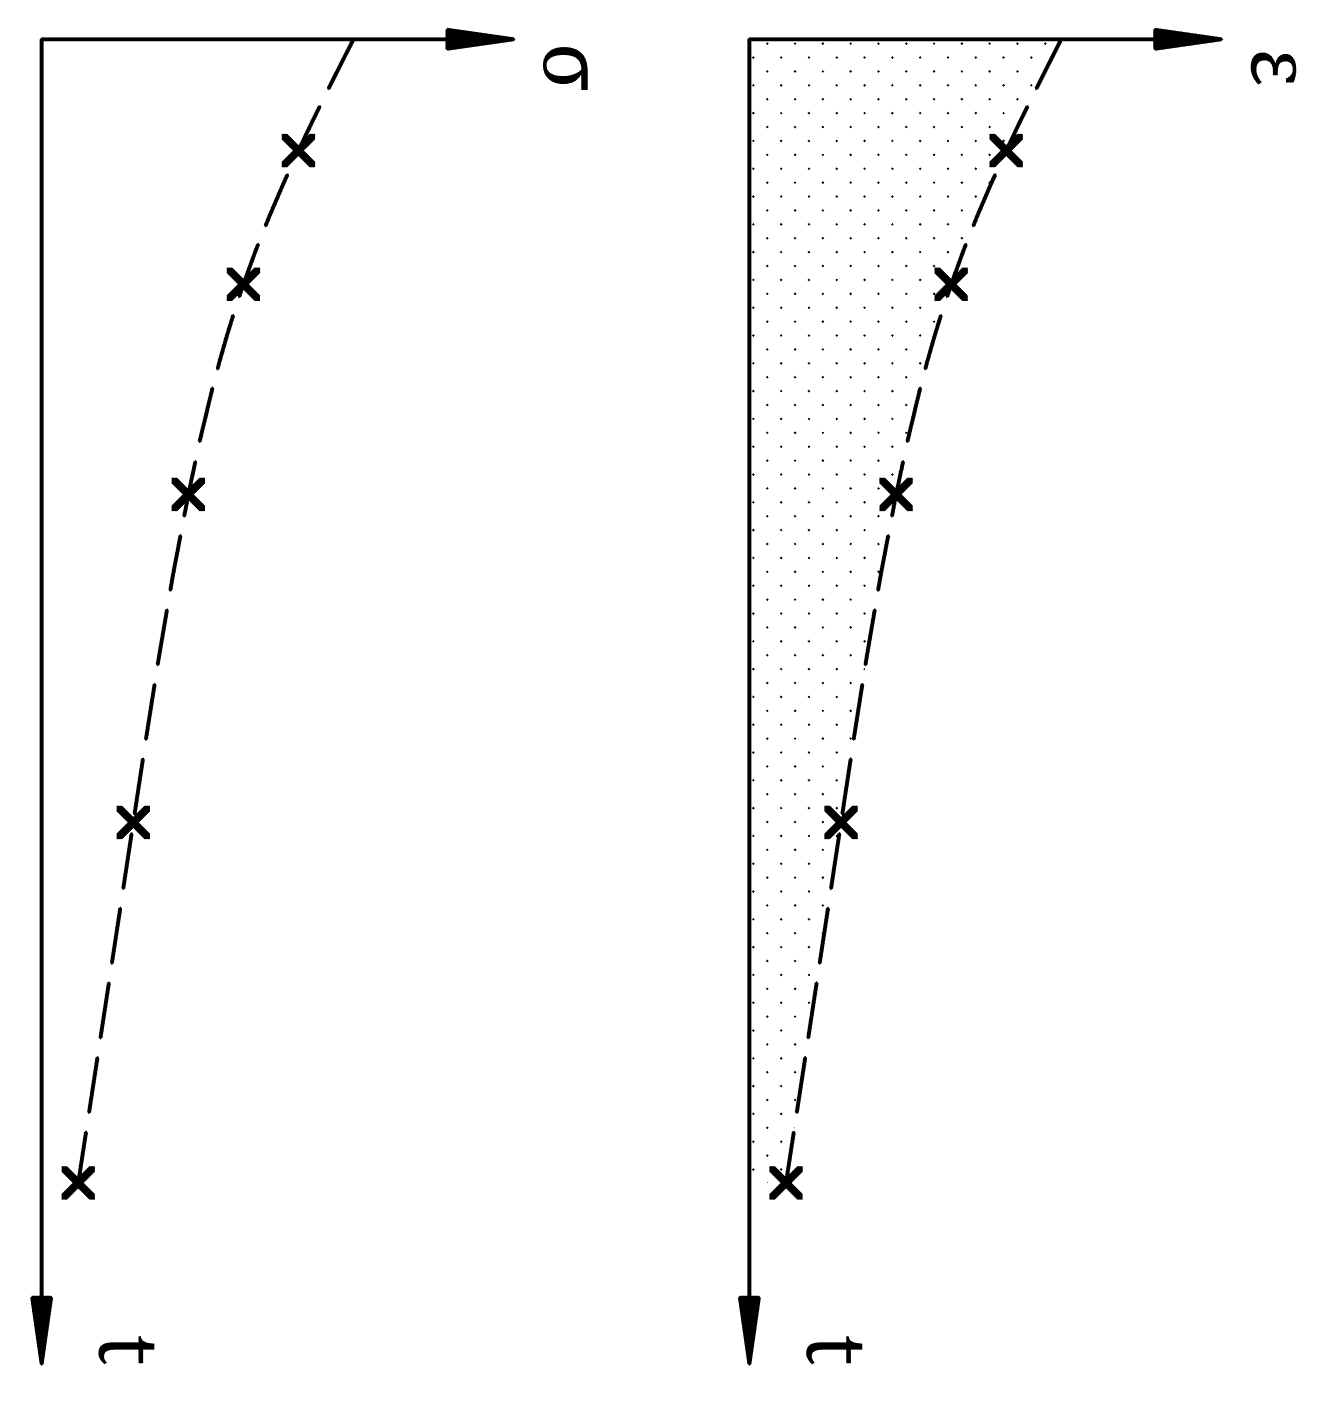
\includegraphics[width=0.35\linewidth,keepaspectratio]{papers/spannung/Grafiken/Bild5.png}
	\caption{Funktionen der Spannung und Dehnung im Zusammenhang mit der Tiefe}
	\label{fig:Bild5}
\end{figure}

Bei jeder dieser Zusatzspannung geht eine entsprechende Zusatzdehnung des Bodens einher, welche eine Setzung bedeutet.
Im einfachsten Fall kann modellhaft mit
\[
\varepsilon
=
\frac{\sigma}{E}
\]
die Setzung an einem Punkt an der Bodenoberfläche mit
\[
s
=
\int_{0}^{\infty}\varepsilon\enspace dt
\]
berechnet werden mit:
\begin{align*}
	\varepsilon &= \text{Dehnung [$-$]}                                     \\
	     \sigma &= \text{Spannung [\si{\kilo\pascal}]}                      \\
	          E &= \text{Elastizitätsmodul; Young-Modul [\si{\kilo\pascal}]}\\
	          t &= \text{Tiefe [\si{\meter}]}                               \\
	          s &= \text{Setzung, Absenkung [m].}
\end{align*}
Diese Zusammenhänge sind wie erwähnt unter anderem im  Lehrbuch [\cite{spannung:Grundlagen der Geotechnik}] beschrieben.
In der praktischen Geotechnik wird man allerdings weitaus schwierigere Situationen antreffen.
Ein Beispiel wäre eine Baugrube mit einem Baugrubenabschluss, wo ein Teil des Bodens abgetragen ist (siehe Abbildung 1.3).
Die Ausbreitung der Zusatzspannung $\sigma(x,y,t)$ würde hier deutlich komplizierter ausfallen.
Dies bedeutet auch eine komplexere Setzung der Bodenoberfläche infolge einer Flächenlast $\sigma$.
Aus allen zusätzlichen Spannungen müssen die adäquaten Dehnungen mit Hilfe einer Spannungsgleichung berechnet werden.
Diese beruht auf Annahmen nach Hooke auf einem linear-elastischen Boden.
Generell wird im Ingenieurwesen versucht Phänomene möglichst nach dem Hook'schen Gesetz abbilden zu können.

\begin{figure}
	\centering
	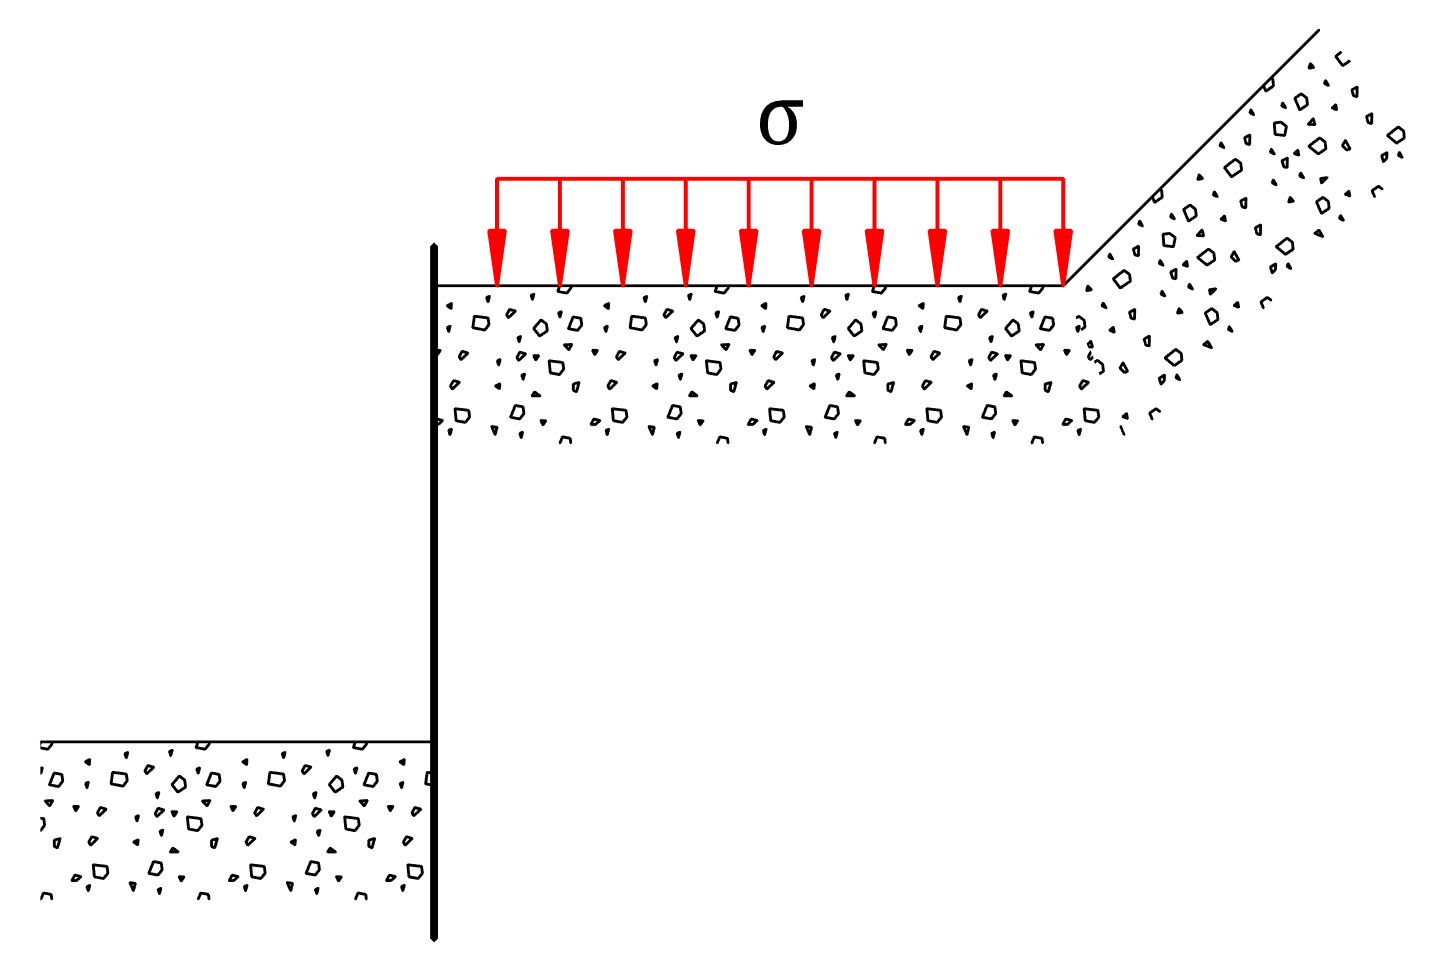
\includegraphics[width=0.45\linewidth,keepaspectratio]{papers/spannung/Grafiken/Bild3.png}
	\caption{Beispiel eines Lastauftrags auf den Boden bei einer komplexeren Situation, welches kompliziertere Spannungsausbreitung zur Folge hat}
	\label{fig:Bild3}
\end{figure}